
\chapter{Vocabulary Tree}
\section{Bag-of-Words模型简介}
解释清楚什么是视觉词汇
\section{TF-IDF}
解释清楚TF-IDF中IDF的含义


\section{DBoW2}
\subsection{TemplateVocabulary}
\begin{figure}[h]%%图
	\centering  %插入的图片居中表示
	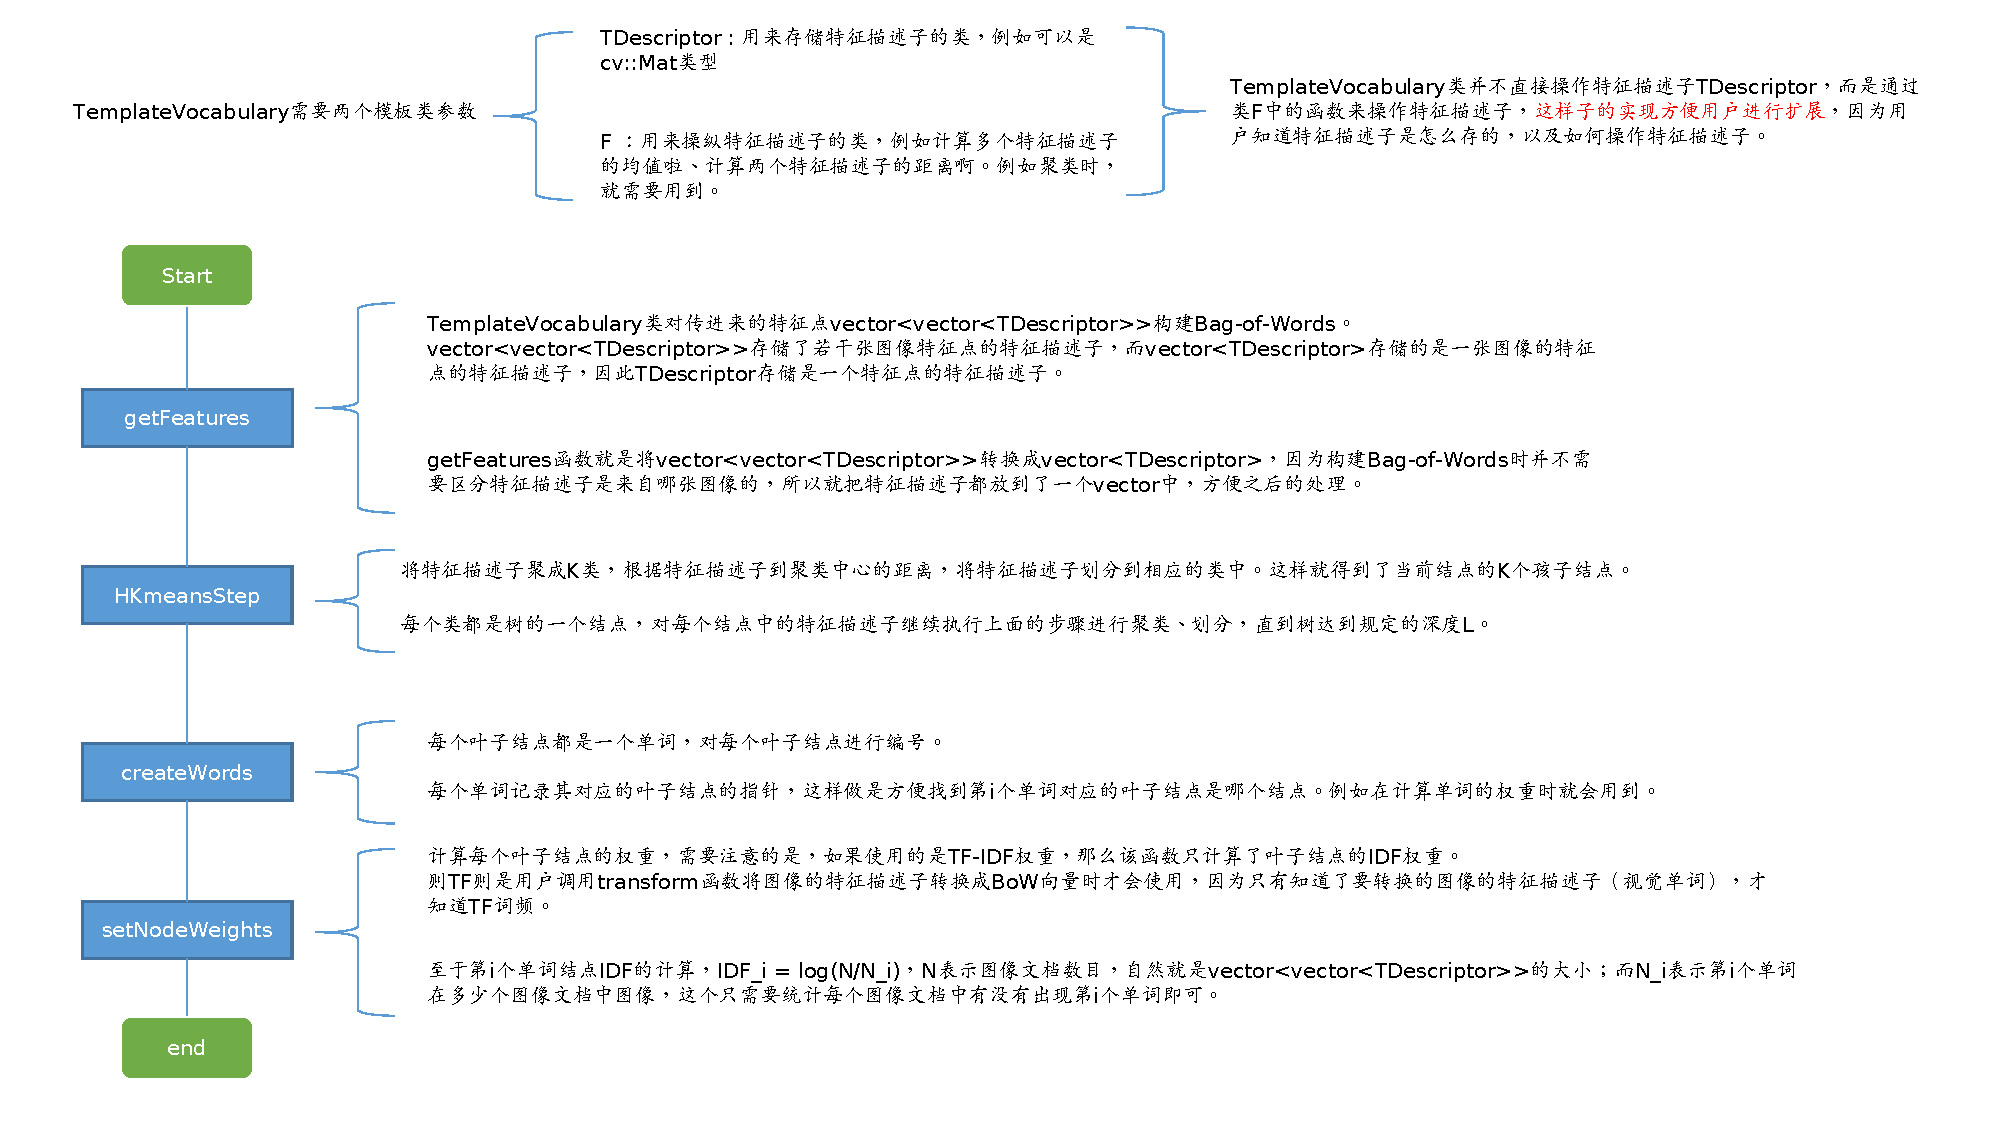
\includegraphics[width=1.0\linewidth]{image/DBoW2/DBoW2.pdf}  %插入的图,包括JPG,PNG,PDF,EPS等,放在源文件目录下
	\caption{词汇树构建流程.}  %图片的名称
\end{figure}


\subsection{BowVector}
建立完词汇树之后,可以将图像(特征描述子)转成BowVector表示,通过表示两个BoWVector的相似性从而得到两张图像的相似性,又因为比较两个BoWVector的速度很快,所以判断两张图片是否相似也就很快了。

构建完词汇树后,用户可以调用TemplateVocabulary的transform函数将图像转换成BoWVector表示(transform函数接受图像的特征描述子作为参数)。由于一般图像只有\textbf{几百}到\textbf{几千}个特征描述子,而词汇树种的叶子结点有\textbf{几百万}到\textbf{几千万}个,所以图像的BoWVector是稀疏向量,所以若直接用向量形式来表示,那么非常浪费空间,效率也不高。所以DBoW2使用STL中的map容器来存储这个向量。map容器中的key表示单词的id,而value则表示该单词的权重,该单词的权重为TF-IDF,其中TF为该单词在图像中出现的频率,而IDF则建树时,叶子结点根据训练集计算得到的权重。

将图像转为BoWVector表示之后,图像之间的相似性就表现为两个BoWVector的相似性。一般来说,图像的BoWVector都经过了L1范数归一化,并且计算相似性时也是使用两个BoWVector之间的L1范数。由于两个经过L1规范化的向量$v$和$w$差的L1范数$||v-w||_1$的范围在[0,2]之间,所以乘以一个$\frac{1}{2}$将其变到[0,1]之间。又因为我们想要L1范数越大表示两张图像越相似,所以将其变成$1 - \frac{1}{2}||v - w||_1$。

计算两个BoWVector之间的L1范数的公式如下:
\begin{eqnarray}
	||v - w||_1 = \sum_i^n |v_i - w_i|
\end{eqnarray}

由于BoWVector$v$和$w$是稀疏向量,上面的计算公式效率太低了,因此要对其进行优化。

对于$v_i$不为0且$w_i$不为0的情况,我们仍旧采用上面的公式进行计算:
\begin{equation}
	||v - w||_1 = \sum_i^n |v_i - w_i| \ , \ for \ all \ i \ and \ v_i \ne 0 \ and \ w_i \ne 0
\end{equation}


对于$v_i$不为0但$w_i$为0的情况:

\begin{equation}
\begin{split}
& ||v = w||_1  = \sum_i^n |v_i - w_i| = \sum_i^n |v_i| \ , \ for \ all \ i \ and \ v_i \ne 0 \ and \ w_i = 0 \\
& = 1 -  \sum_i^n |v_i|, for \ all \ i \ and \ v_i \ne 0 
\end{split}
\end{equation}


同理,对于$v_i$为0但$w_i$不为0的情况:

\begin{equation}
\begin{split}
& ||v = w||_1  = \sum_i^n |v_i - w_i| = \sum_i^n |w_i| \ ,\ for \ all \ i \ and \ v_i = 0 \ and \ w_i \ne 0 \\
& = 1 -  \sum_i^n |w_i| \ , for \ all \ i \ and \ w_i \ne 0 
\end{split}
\end{equation}

综上,得到:
\begin{equation}
	||v - w||_1 = 2 + \sum_i^n |v_i - w_i| -|v_i| - |w_i|  \ ,\ for \ all \ i \ and \ v_i \ne 0 \ and \ w_i \ne 0 \\
\end{equation}



所以,在计算两个BoWVector的相似性时,由于BoWVector使用STL的map进行存储,map容器中的key表示单词的id,而value则表示该单词的权重。所以只需要找到两个map中key相同的元素,进行上面的计算即可。实际的代码如下:

\begin{lstlisting}[language = C++]
double L1Scoring::score(const BowVector &v1, const BowVector &v2) const
{
	BowVector::const_iterator v1_it, v2_it;
	// 得到两个BoW向量的迭代器,实际上是map容器的迭代器
	const BowVector::const_iterator v1_end = v1.end();
	const BowVector::const_iterator v2_end = v2.end();
	
	v1_it = v1.begin();
	v2_it = v2.begin();
	
	double score = 0;
	
	while(v1_it != v1_end && v2_it != v2_end)
	{
		const WordValue& vi = v1_it->second;
		const WordValue& wi = v2_it->second;
		
		// 当两个BoW向量中,相同单词的权重都不为空时,根据公式进行计算
		if(v1_it->first == v2_it->first)
		{
			score += fabs(vi - wi) - fabs(vi) - fabs(wi);
			
			// move v1 and v2 forward
			++v1_it;
			++v2_it;
		}
		else if(v1_it->first < v2_it->first)
		{
			// move v1 forward
			v1_it = v1.lower_bound(v2_it->first);
			// v1_it = (first element >= v2_it.id)
		}
		else
		{
			// move v2 forward
			v2_it = v2.lower_bound(v1_it->first);
			// v2_it = (first element >= v1_it.id)
		}
	}
	
	// ||v - w||_{L1} = 2 + Sum(|v_i - w_i| - |v_i| - |w_i|) 
	//		for all i | v_i != 0 and w_i != 0 
	// (Nister, 2006)
	// scaled_||v - w||_{L1} = 1 - 0.5 * ||v - w||_{L1}
	score = -score/2.0;
	
	return score; // [0..1]
}


\end{lstlisting}


\subsection{FeatureVector}
我们知道闭环检测时,需要知道找到与当前关键帧相似的图像帧,
BowVector的作用在于快速判断两张图像的相似性;在找到相似的图像之后,需要做的就是找到两张图像中特征点的匹配关系,这当然可以使用KDTree来办到,但是这太慢了(要先对一张图像的特征点构建KDTree,另一张图像才能使用特征点进行查询),DBoW2的作者使用FeatureVector来实现快速找到两张图像中特征点的匹配关系。


我们知道图像的每个特征点对应了哪个叶子结点,那么也就知道了哪个叶子结点id对应了哪个特征描述子,所以类似BowVector的原理,对于FeatureVector也使用STL的map进行存储,其中key表示叶子结点的id,value表示经过该叶子结点的特征描述子(的id),那么接下来的比较就是类似BoW向量的比较,只需要比较两个FeatureVector(两个map)中具有相同叶子结点id的那些特征描述子。由于不同的特征描述子可能经过同一个叶子结点,所以FeatureVector的实际结构是这样的:FeatureVector类继承了std::map<int, std::vector<unsigned int>>类,其中key表示结点的id(不一定是叶子结点id),std::vector<unsigned int>表示经过该结点的特征描述子都有哪些。

之前不是说map的key表示叶子结点的id,那么为什么现在又说key表示的不一定是叶子结点的id呢?这是为了提高特征匹配的正确性,
由于词汇树可能划分地太细了,可能导致两个相似的特征描述子被分在了两个相邻的叶子结点上,若是我们只要相同的叶子结点上进行特征描述子的比较,那么就会错过正确的匹配。但是我们发现,虽然它们被分在了相邻的叶子结点,但是它们经过了同一个父亲结点啊,由于词汇树的特性,两个特征描述子只要经过了相同的结点,那么其就有可能是正确的匹配。为了提高鲁棒性,现在FeatureVector的map中的key存储的不再是叶子结点的id(倒数第一层结点的id),可能是倒数第二层、第三层结点的id(ORB-SLAM2使用的是倒数第四层的,可能是经过了一些测试采用的吧),而value则表示经过那些结点的特征描述子有哪些。至于比较过程,还是只需比较具有相同结点id的那些特征描述子即可。


\subsection{TemplateDatabase}
如果我们想在n张图像中找到与查询图像相似的图像该怎么办?如果使用TemplateVocabulary,那么就是讲n张图像和查询图像转换成BoWVector表示,然后对于n张图像中的每张图像和查询图像之间利用BoWVector计算相似性,然后按照相似性,找到相似图像。


TemplateDatabase的作用就是用来快速在一堆图像中找到与查询图像相似的图像的。

构造TemplateDatabase时,需要传入一个词汇树(构造好的TemplateVocabulary对象);然后需要不断调用add函数,将图像的特征描述子添加到TemplateDatabase中,该函数构建了图像的invert list,也即记录了每个叶子结点都被哪张图像的特征描述子经过。

在查询时,只需要遍历查询图像的BoWVector,然后通过invert list累积相应图像的评分,最终哪张图像的评分最高,那么哪张图像就与查询图像最相似。



\section{参考文献}
DBoW2算法原理 http://www.cnblogs.com/jian-li/p/5664559.html
